\section{When to Use @ngrx/store}
When to use @ngrx/store can be a very opiniated item to consider. State as we
know it, is a single data object, that can be accessed anywhere within the app.
How this happens, changes from one state management framework to another, but
the core is the same. However, the difficulty, is that state, being that it
exists outside of the component, can contain quite a bit of bloat.

\mybox{It is interesting to note, that the original implementation of Flux
was created by Facebook back in 2014\footnote{This \href{https://www.youtube.com/watch?v=nYkdrAPrdcw}{video} contains this fact}.
It was because they had a bug with regards to the chat counter, that just kept
on coming back. It would mention that a user did not read a message, but that
wasn't true. Flux was the architecture they came up with in order to solve this
bug. It's important to understand the history of where Flux came from, when
trying to understand how to move forward using it. It's important to also
realize, that the issue, wasn't they weren't able to solve it, it is that the
bug kept coming back. Flux solved it, due to it's straight forward way of
solving multiple components interacting with each other.

``It is important to remember, that a store is about creating an in-memory client
side database, which is a user-specific slice of the database, and use that
data to derivce View Models from it on the client.''
}

\subsection{Redux as evolution on Flux}
Redux solved the same problem Flux did. However, it simplified the process.
Without going into too much detail and instead showing a photo, Redux simplified
the problem it solved, and made it easier to implement:

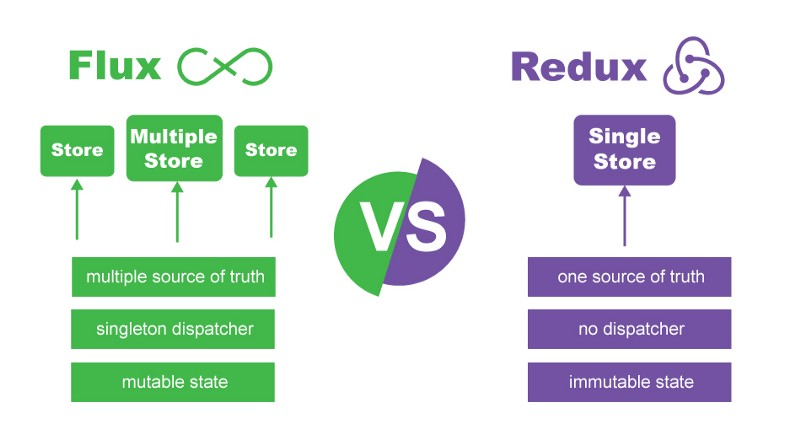
\includegraphics[width=9.1cm, height=6cm]{./state/when-to-use-ngrx/flux_v_redux}

It also more importantly, standardized the Flux architecture as a library.

\subsection{@ngrx/store - Integrated Reactive Programming with the Store}
@ngrx/store took redux one step further, and integrated observables with the
store. There is a fantastic founding paper on the benefits of Real Time:
\href{http://www-sop.inria.fr/members/Gerard.Berry/Papers/Berry-IFIP-89.pdf}{Programming}

In it, it discusses two main benefits of Reactive Programming:
\begin{enumerate}
  \item Asynchronous
  \item Detemrinistic
\end{enumerate}

Just to throw out what a quote from who I consider a founder in Reactive
programmin. Andre Staltz when discussing why one should consider Reactive
programming really touches on the core of it all with the following, "Reactive
Programming raises the level of abstraction of your code so you can focus on 
the interdependence of events that define the business logic\ldots".
\footnote{https://gist.github.com/staltz/868e7e9bc2a7b8c1f754\#why-should-i-consider-adopting-rp}

That being said, it immediately becomes obvious as to why one would want a
reactive approach towards state. State is generally changed with events, and
being able to abstract the level of state makes complete sense. I cannot stress
how many times, I have been able to pull in an observable using @ngrx/store, and
modify it using rxjs. It greatly abstracts, and simplifies the process.

\mybox{As a side note, ngrx was actually created, to solve performance issues
with change detection in Angular2. It from that point onwards has morphed into
a good idea, allowing the store to be automatically hooked into state:
https://github.com/ngrx/store/issues/16\#issuecomment-172027797}

\subsection{ An Example of an @ngrx/store }

For instance, let's say that we have a user-settings data-access feature. Our
folder file structure might look like the following:

\begin{forest}
  [libs
    [px-illustrator
      [data-access
        [user-settings
          [src
            [lib
              [\_+state
                [\_user-settings.actions.ts,file]
                [\_user-settings.effects.spec.ts,file]
                [\_user-settings.effects.ts,file]
                [\_user-settings.facade.mock.ts,file]
                [\_user-settings.facade.spec.ts,file]
                [\_user-settings.facade.ts,file]
                [\_user-settings.reducer.spec.ts,file]
                [\_user-settings.reducer.ts,file]
                [\_user-settings.selectors.ts,file]
              ]
              [\_px-illustrator-data-access-user-settings.module.ts,file]
              [\_px-illustrator-data-access-user-settings.module.spec.ts,file]
              [\_px-illustrator-data-access-user-settings-testing.module.spec.ts,file]
            ]
            [\_index.ts,file]
            [\_test.ts,file]
          ]
          [\_karma.conf,file]
          [\_README.md,file]
          [\_tsconfig.lib,file]
          [\_tsconfig.lib.json,file]
          [\_tsconfig.spec.json,file]
          [\_tslint.json,file]
        ]
      ]
    ]
  ]
\end{forest}


This, of course, would be in an enterprise setting, which honestly this book
is geared towards. However, it definitely strikes home a very good point. There
is a ton of bloat to creating a store. Even once a developer get's over the hill
of creating state, and get's used to it, it's still a lot to manage, and one
just has to ask, does it always make sense?

\subsection{Understanding the Reality of State}
I think that looking at the above folder/file strucutre, it is very important
to realize that state has gone so far beyond what it was originally intended to
do. You will notice effects, a facade pattern. In addition, quietly sitting
inside of our reducer, is @ngrx/entity. The whole suite of @ngrx is so robust
that it deals with the entire life cycle, of pulling in data, and integrating it
with the client side. In fact, if it wasn't for the bloat that it introduced,
it would be able to solve every single situation, wherein we are trying to carry
over data into the client side, in a scalable, and maintainable fashion. Ok, so
let's deep dive into it.

\subsection{ Addressing the Problems State Alleviates }
First and foremost, I think it would be most effective if we were to directly
jump into the problems that state solves:
\begin{enumerate}
  \item Avoiding Multiple Actors
  \item Avoid Extraneous @Inputs
  \begin{enumerate}
    \item Pass down multiple levels to child, and send change back to parent
    \item Siblings in a tree, might have to pass up and over
  \end{enumerate}
  \item Stops Event Bussing /marginpar{Look more into this one}
  \item Decouples component interaction. Component does not know what changed,
  only knows what changed it.
  \item Allows for Component interaction via the Observable Pattern
  \item Client Side Cache if needed.
  \item Place to Put Temporary UI State
\end{enumerate}

These would be in my humble opinion, the 7 things that state has to offer. If a
component were to be able to interact with another component on that page, by
altering it's data, it should have state.

\subsubsection{ Addressing Additional two Offered by @ngrx/store }
Added into your classic @nrwl/nx ecosystem, is:
\begin{enumerate}
  \item @ngrx/entity
  \item Facade pattern for single
  \item Effects for asynchronous programming
\end{enumerate}

\subsection{The Mesmerism of @ngrx/store}

So, as mentioned before, the @ngrx/store ecosytem has grown into a beast. In
fact, an Angular developer working on an enterprise, data heavy application,
might spend 60\% to 70\%(rough estimate) of their time working within
@ngrx/store. I was a little bit curious as to how this repition might
psychologically affect the way that we as software engineers develop. In
particular, if we can introduce services that accomplish what @ngrx/store does,
albeit less bloat, is it worth it for the team?

I found an interesting book, called, ``On Repeat: How Music Plays the Mind''. It
discusses a very interesting topic, of how we as humans interact with music. In
it, it discusses something known as ``The Exposure Effect''. It's something that
we have all experienced with regards to music. For instance, you will hear some
music on the radio that you are not particularly fond of. However, you will here
it again the grocery store, movie theater, and then the store corner once again!
By this time, you are hooked! More importantly, as the book discusses, as you
are used to the repition of the song, you are already expecting the next piece
of song, by the time you working on the beginning of it. Repition, allows for us
as the book argues, to look at a passage as a whole.

Arguably, the point can be made for software as well. Within the application you
are working on, the more you use that pattern the more accustomed you are to it.
In addition, and I can personally attest to this, by the time, I am working on
the facade, I am already thinking of the effect that is going to tie into our
service, and how I am going to tie it into the component. Jumping out of this
repitition can counter-productive, even if there is less code involved by
creating a service.

\subsection{ Attachments Service - Story Time }
There are some very unique cases, where perhaps state shouldn't be used on an
objective level. I for one always felt that state has a bit of bloat(, albeit my
opinion is beggining to change). However, after discussing with team members,
I have begun to see the way they think. This particular situation was about a
feature for attachments that the app needed. In particular, multiple components
on the same page, would have attachments that would be uploaded to a server.
Then, when the api using the attachment would make a request, it would pull
attachment from the server, using it's id. If a service or @ngrx/store was not
used, there would be alot of repitition across the app. This led to the dillema,
should a service, or @ngrx/store be used.

\subsection{ Business Requirements }
One, is that multiple components on the same page were to use this attachments
service. Second, is that we want to show the user when a certain attachment is
loading, and when it is no longer loading.

\subsection{ Argument for using a Service }
In truth, the attachments were meant to be self contained within a singular
component. This would have made the service as very simple. However, based on
the business requirements, we would have had to create a double nested
correlation id. This means that a double nested correlation id pattern had to be
created. One, to make sure that different components do not affect each other.
Two, the id produced on the front end, is different than the id produced on the
backend. We need to create an id that can be used by both. This is done by
creating a second Uuid, that is nested within the first one. I.e. a dictionary
inside of a dictionary.

So, really in this situation, there is arguably nothing that the store has to
offer. However, what has happened, using ``The Exposure Effect'' is that we are
now comfortable with the API for @ngrx/entity. Comfortable isn't accurate
actually. We are able to predict, @ngrx/store as a whole. Any developer who
worked and will work within the app, can pick up on the code base easier than
a service, beign that it is predictable. In addition, we have a single place
where we expect all of our data to be. Creating a service like this, might make
sense for the person spending the time thinking through the problem. However,
for any other person, it will be an incredibly uncomfortable experience reading
through your code. @ngrx/store therefore at this point takes on it's new life
as a way to make sure code is consistent, even if it isn't the right choice for
your app.

\subsection{ What Comes Out From Our Back and Forth }
Truly, any enterprise situation, wherein a data request is made from the
back end, it should be handled using @ngrx/store and not services. This is
simply because, in any enterprise setting, the majority of situations is more
properly handled using @ngrx/store.
\begin{enumerate}
  \item It allows for a cookie cutter api, that is used time and time again. The
  code bloat it creates, is alleviated by use of Nrwl Nx.
  \item Your application's performance will not affected as a result.
  \item From personal experience, business requirment change quite a bit. The
odds of your service now being needed to re-written to accomodate it being
used in multiple components, is also quite high.
\end{enumerate}

\subsection{ Final Note }
If you are building an enterprise app from the beginning and are building a
team, put this as part of the conventions right away. It will make your life
easier. If you have a team, and you haven't fully agreed on this one, send them
this article and start a conversation. Razroo Cares.
